\documentclass[journal, a4paper]{IEEEtran}
\usepackage[T1]{fontenc}       % Encodage le plus étendu
\usepackage[utf8]{inputenc}    % Source Unicode en UTF-8

\usepackage[cyr]{aeguill}
\usepackage[francais]{babel} % Pour la redaction du document en francais


% some very useful LaTeX packages include:

%\usepackage{cite}      % Written by Donald Arseneau
                        % V1.6 and later of IEEEtran pre-defines the format
                        % of the cite.sty package \cite{} output to follow
                        % that of IEEE. Loading the cite package will
                        % result in citation numbers being automatically
                        % sorted and properly "ranged". i.e.,
                        % [1], [9], [2], [7], [5], [6]
                        % (without using cite.sty)
                        % will become:
                        % [1], [2], [5]--[7], [9] (using cite.sty)
                        % cite.sty's \cite will automatically add leading
                        % space, if needed. Use cite.sty's noadjust option
                        % (cite.sty V3.8 and later) if you want to turn this
                        % off. cite.sty is already installed on most LaTeX
                        % systems. The latest version can be obtained at:
                        % http://www.ctan.org/tex-archive/macros/latex/contrib/supported/cite/

\usepackage{graphicx}   % Written by David Carlisle and Sebastian Rahtz
                        % Required if you want graphics, photos, etc.
                        % graphicx.sty is already installed on most LaTeX
                        % systems. The latest version and documentation can
                        % be obtained at:
                        % http://www.ctan.org/tex-archive/macros/latex/required/graphics/
                        % Another good source of documentation is "Using
                        % Imported Graphics in LaTeX2e" by Keith Reckdahl
                        % which can be found as esplatex.ps and epslatex.pdf
                        % at: http://www.ctan.org/tex-archive/info/

%\usepackage{psfrag}    % Written by Craig Barratt, Michael C. Grant,
                        % and David Carlisle
                        % This package allows you to substitute LaTeX
                        % commands for text in imported EPS graphic files.
                        % In this way, LaTeX symbols can be placed into
                        % graphics that have been generated by other
                        % applications. You must use latex->dvips->ps2pdf
                        % workflow (not direct pdf output from pdflatex) if
                        % you wish to use this capability because it works
                        % via some PostScript tricks. Alternatively, the
                        % graphics could be processed as separate files via
                        % psfrag and dvips, then converted to PDF for
                        % inclusion in the main file which uses pdflatex.
                        % Docs are in "The PSfrag System" by Michael C. Grant
                        % and David Carlisle. There is also some information
                        % about using psfrag in "Using Imported Graphics in
                        % LaTeX2e" by Keith Reckdahl which documents the
                        % graphicx package (see above). The psfrag package
                        % and documentation can be obtained at:
                        % http://www.ctan.org/tex-archive/macros/latex/contrib/supported/psfrag/

%\usepackage{subfigure} % Written by Steven Douglas Cochran
                        % This package makes it easy to put subfigures
                        % in your figures. i.e., "figure 1a and 1b"
                        % Docs are in "Using Imported Graphics in LaTeX2e"
                        % by Keith Reckdahl which also documents the graphicx
                        % package (see above). subfigure.sty is already
                        % installed on most LaTeX systems. The latest version
                        % and documentation can be obtained at:
                        % http://www.ctan.org/tex-archive/macros/latex/contrib/supported/subfigure/

\usepackage{url}        % Written by Donald Arseneau
                        % Provides better support for handling and breaking
                        % URLs. url.sty is already installed on most LaTeX
                        % systems. The latest version can be obtained at:
                        % http://www.ctan.org/tex-archive/macros/latex/contrib/other/misc/
                        % Read the url.sty source comments for usage information.

%\usepackage{stfloats}  % Written by Sigitas Tolusis
                        % Gives LaTeX2e the ability to do double column
                        % floats at the bottom of the page as well as the top.
                        % (e.g., "\begin{figure*}[!b]" is not normally
                        % possible in LaTeX2e). This is an invasive package
                        % which rewrites many portions of the LaTeX2e output
                        % routines. It may not work with other packages that
                        % modify the LaTeX2e output routine and/or with other
                        % versions of LaTeX. The latest version and
                        % documentation can be obtained at:
                        % http://www.ctan.org/tex-archive/macros/latex/contrib/supported/sttools/
                        % Documentation is contained in the stfloats.sty
                        % comments as well as in the presfull.pdf file.
                        % Do not use the stfloats baselinefloat ability as
                        % IEEE does not allow \baselineskip to stretch.
                        % Authors submitting work to the IEEE should note
                        % that IEEE rarely uses double column equations and
                        % that authors should try to avoid such use.
                        % Do not be tempted to use the cuted.sty or
                        % midfloat.sty package (by the same author) as IEEE
                        % does not format its papers in such ways.

\usepackage{amsmath}    % From the American Mathematical Society
                        % A popular package that provides many helpful commands
                        % for dealing with mathematics. Note that the AMSmath
                        % package sets \interdisplaylinepenalty to 10000 thus
                        % preventing page breaks from occurring within multiline
                        % equations. Use:
%\interdisplaylinepenalty=2500
                        % after loading amsmath to restore such page breaks
                        % as IEEEtran.cls normally does. amsmath.sty is already
                        % installed on most LaTeX systems. The latest version
                        % and documentation can be obtained at:
                        % http://www.ctan.org/tex-archive/macros/latex/required/amslatex/math/

\usepackage{lipsum} % Dummy text


% Other popular packages for formatting tables and equations include:

%\usepackage{array}
% Frank Mittelbach's and David Carlisle's array.sty which improves the
% LaTeX2e array and tabular environments to provide better appearances and
% additional user controls. array.sty is already installed on most systems.
% The latest version and documentation can be obtained at:
% http://www.ctan.org/tex-archive/macros/latex/required/tools/

% V1.6 of IEEEtran contains the IEEEeqnarray family of commands that can
% be used to generate multiline equations as well as matrices, tables, etc.

% Also of notable interest:
% Scott Pakin's eqparbox package for creating (automatically sized) equal
% width boxes. Available:
% http://www.ctan.org/tex-archive/macros/latex/contrib/supported/eqparbox/

% *** Do not adjust lengths that control margins, column widths, etc. ***
% *** Do not use packages that alter fonts (such as pslatex).         ***
% There should be no need to do such things with IEEEtran.cls V1.6 and later.


% En-tête et pied de page
%\usepackage{lastpage}
%\usepackage{fancyhdr}
%\pagestyle{fancy}
%\renewcommand{\sectionmark}[1]{\markright{#1}}
%\fancyhead{}
%%\fancyhead[RO,LE]{\slshape\footnotesize\nouppercase{\rightmark}}
%\fancyhead[LO,RE]{\thetitle}
%\fancyfoot{}
%%\fancyfoot[LO,RE]{\footnotesize\texttt{\thefilename}\\ \textit{\now}}
%%\fancyfoot[C]{-~\thepage~/~\pageref{LastPage}~-}
%\fancyfoot[RO,LE]{\raisebox{-2mm}{\includegraphics{structure/barrette-original}}}
%%
%\fancypagestyle{plain}{ %  Première page ----------------------
%  \fancyhead{}
%  \renewcommand{\headrulewidth}{0pt}
%  \fancyheadoffset[R]{15mm}
%  \fancyhead[L]{
%    \raisebox{-7mm}{
%      \parbox{\textwidth}{
%        \includegraphics{structure/barrette-original} \\ \\
%        \fontsize{8pt}{10pt}\selectfont
%        \sffamily\color{Pantone287}
%        FACULTÉ DES SCIENCES       \\
%        DÉPARTEMENT D'INFORMATIQUE
%      }
%    }
%  }
%  \fancyhead[R]{
%    \raisebox{-10mm}[0pt][0pt]{\includegraphics[width=120mm]{structure/ULB-ligne-gauche}}
%  }
%  \fancyfoot{}
%  %\fancyfoot[L]{\raisebox{0mm}{}\color{Pantone287}\footnotesize\texttt{\thefilename}\\ \textit{\now}}
%  %\fancyfoot[C]{-~\thepage~/~\pageref{LastPage}~-}
%  \fancyfoot[R]{
%    \raisebox{-12pt}{\includegraphics[height=\footskip]{structure/sceau-mini-b-quadri}}
%  }
%} % Fin de première page
% ---------------------------------------------------------------------------


% Your document starts here!
\begin{document}

% Define document title and author
	\title{Modélisation de la vaccination des individus et de la population dans le cadre d'une épidémie}
	\author{Nathan Marotte
	\thanks{Superviseurs: Robin Petit}}
	\markboth{INFO-F308}{}
	\maketitle

% Write abstract here
\begin{abstract}
	Le vaccin est un sujet souvent débattu car son efficacité n'est pas ressentie de la même manière qu'un antibiotique ou qu'un anti-douleur. Nous allons montrer dans cet article, par des modèles et simulations simple, comment un vaccin altère la propagation d'une maladie, au-delà de la protection qu'il apporte à un individu, en créant une véritable barrière qui rend la population presque immunisée si un certain pourcentage de la population est vacciné.
\end{abstract}

% Each section begins with a \section{title} command
\section{Introduction}
	\PARstart{L}{e} monde étant rempli de sceptiques, les vaccins ont reçu et reçoivent encore bon nombre de critiques sur leur efficacité et donc autant de personnes refusant de ce faire vacciner. Les taux d'exemptions non médicales des vaccins varient d'une population à l'autre mais aurait atteint jusque 26.67\% \cite{NME_vaccine} dans certaines populations. Comme nous le verrons plus loin, toutes ces personnes contribuent à une augmentation du risque d'épidémie, un anéantissement du phénomène d'immunité collective, et mettent en danger la vie des individus ne pouvant pas être vaccinés pour raisons médicales (allergies, ...).\

	Cet article aura donc pour but de défendre la vaccination en simulant la propagation d'une épidémie dans une population vaccinée à un certain pourcentage afin de voir comment le taux de vaccination dans une population influence de manière \emph{non linéaire} l'immunité de la maladie. Cette relation est aussi connue sous le nom d'immunité grégaire ou \emph{herd immunity, en anglais}.
	Trouver le seuil de cette immunité, c'est-à-dire le taux de vaccination nécéssaire pour qu'un malade transmette la maladie à moins d'une personne en moyenne, permettra de déterminer quelles populations sont potentiellement en danger d'épidémies graves, et de pouvoir nous concentrer sur celles-ci afin d'éviter d'autres catastrophes. Ce seuil est appellé \emph{Herd Immunity Threshold}, ou \emph{HIT}
	Notre approche fournira à la communauté scientifique des méthodes très simples et compréhensibles, mais correctes pour démontrer au public les raisons de la vaccination obligatoire.

	\subsection{Lexique}
	Nous allons ici définir les termes utilisés dans cet article
	\begin{itemize}
		\item Un modèle est un outil permettant de représenter la réalité de manière mathématique
		\item Une simulation est l'exécution d'un programme informatique sur un modèle afin d'obtenir un résultat
		\item Un état d'un modèle est une situation dans laquelle se trouve un individu du modèle
		\item Une transition dans un modèle est le lien entre 2 états. Elle est souvent associée à une probabilité de suivre cette transition, c'est à dire de passer de l'état à la base de la transition vers l'état au bout de la transition
		\item Un modèle est dit compartimental si il est uniquement représenté par le nombre d'individu dans chaque état du modèle
		\item Un modèle est dit spatial si il est représentable schématiquement, sous forme matricielle par exemple. Chaque individu est donc modélisé à part entière
	\end{itemize}
	Nous allons aussi expliquer ici comment le modèle compartimental SIR fonctionne. \\
	SIR est un des modèles épidémiologique les plus simples. Il est composé de 3 états et de maximum 3 transitions (une entre chaque état). Chaque lettre représente un état, ici Susceptible (sain et infectable), Infecté (malade et contagieux), et Retiré (guéri ou mort). Les 3 transitions sont les probabilité d'être infecté (S->I), probabilité de mourir/guérir (I->R) et probabilité de perdre l'immunité (dans le cas où R est guéri et non mort) (R->S)

\section{Etat de l'art}
	Le modèle étant par nature assez simple, peu d'articles récents ont été écrits sur le sujet, il existe cependant ces quelques articles avec un modèle proche de SIR
	\subsection{Grippe saisonnière}
		L'article \cite{pandemic_influenza} a pour but d'expliquer l'utilisation des modèles et de déterminer les conditions qui peuvent être utilisées pour évaluer l'efficacité des vaccins, entre autre. \\
		Il présente un modèle $SI_{tr}I_uRV$ pour la modélisation de la grippe saisonnière. Un individu commence susceptible et peut être vacciné à un certain temps, ou bien infecté et traité, ou infecté et pas traité. Dans les deux cas, l'individu finira par être guéri au final (plus ou moins vite selon si il est traité ou pas). Le diagramme de transition est présenté en figure \ref{fig:pandemic_influenza_model}
		\begin{figure}[!hbt]
			\caption{Diagramme de transition entre les différents états du modèle}
			\includegraphics[width=\columnwidth]{pandemic_influenza_model}
			\label{fig:pandemic_influenza_model}
			\cite{pandemic_influenza}
		\end{figure} \\


		 L'article \cite{influenza_HIT} quant à lui à pour objectif d'essayer de déterminer le taux de vaccination nécéssaire pour que la population soit protégée par le phénomène d'immunité collective pour les différentes épidémies de 1918/19, 1957/58, 1968/69, 2008/09 et 2009/10. Ces taux de vaccinations sont calculés à partir de la formule \ref{eqn:influenza_formula}

		 \begin{equation}
		 \label{eqn:influenza_formula}
		 	\begin{aligned}
		 		V_c = \frac{I_c}{E} = \frac{1-(\frac{1}{R_0})}{E}
		 	\end{aligned}
		 \end{equation}

		 où $V_c$ est le taux de vaccination nécéssaire, $I_c$ est le seuil d'immunité collective et $E$ le taux d'efficacité du vaccin. Nous utiliserons une formule similaire dans la section \ref{sec:met}, sans prendre en compte l'efficacité du vaccin

	 \subsection{VIH}
	 L'article \cite{Imperfect_vaccines_and_herd_immunity_to_HIV_1993} utilise un modèle a 4 états (Susceptible, Vacciné, Infecté, et SIDA) pour représenter la transmission du SIDA dans la communauté homosexuelle masculine.
	 Des nouvelles personnes peuvent entrer dans le modèle et en sortir, faisant de ce modèle un modèle très réaliste. Le modèle est résumé dans l'article par la figure \ref{fig:hiv_model}. Les transitions entrantes représentent les hommes entrants dans la communauté homosexuelle et les transitions sortantes, les sorties de la commuanuté ainsi que les morts pour les transitions sortantes de l'état SIDA.

	 \begin{figure}[!hbt]
		 \caption{Structure du modèle à SIDA}
		 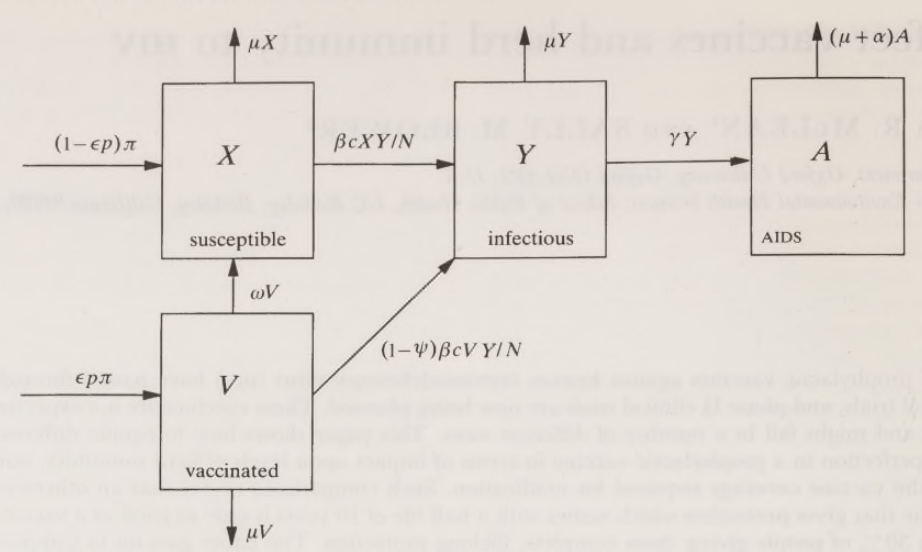
\includegraphics[width=\columnwidth]{Imperfect vaccines and herd immunity to hiv_model}
		 \label{fig:hiv_model}
		 \cite{Imperfect_vaccines_and_herd_immunity_to_HIV_1993}
	 \end{figure}

	 \subsection{Quarantaine et vaccination}
	 Il existe aussi des expériences sur les effets de la prévention (vaccination) et de la quarantaine notamment \cite{Kato2011}. Leur modèle spatial introduit des sites (cases, dans notre simulation) qui sont protégés d'une quelconque infection, considérés donc vaccinés ainsi que des bords (maximum 4 par site non protégés) de cases permettant de bloquer la transmission par ce bord. Ces bordures représentent la quarantaine dans leur modèle. La figure \ref{fig:quarantine_model} tirée de leur article illustre leur modèle spatial
	 \begin{figure}[!hbt]
		 \caption{Représentation du modèle spatial avec quarantaine et immunités}
		 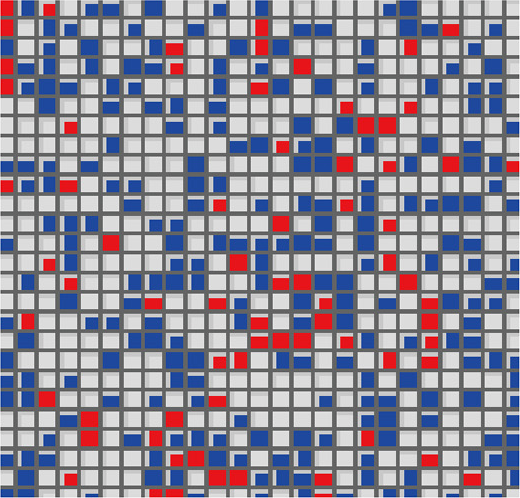
\includegraphics[width=\columnwidth]{quarantine_model}
		 \label{fig:quarantine_model}
		 \cite{Kato2011}
	 \end{figure}




% Main Part
\section{Méthodologie}\label{sec:met}
	Afin d'étayer notre hypothèse, les vaccins protègent au delà du système immunitaire, nous avons construit un modèle SIR simple où la population de départ est repartie dans les différents états pour une représentation compartimentale et nous avons aussi construit une modèle spatial se basant sur les 3 états et les transitions du modèle compartimental SIR.
	Grâce à ces modèles, nous allons pouvoir déterminer le seuil d'immunité grégaire \emph{HIT} mais aussi voir l'évolution de la protection en fonction du nombre de vaccinés.

	Nous avons donc écrit un programme Python qui va générer 500.000 populations de 2500 individus chacun. Chaque population aura un taux de vaccination de telle sorte qu'il y aura 5000 populations par pourcentage de vaccination (entre 0 et 99\%). Ensuite nous faisons la moyenne du nombre de personnes qui n'étaient pas vaccinés et qui n'ont pas été touchées par la maladie (en excluant des calculs le patient zéro), en regroupant les populations par taux de vaccination. Nous allons voir dans cette section tout ce qui nous a permis à implémenter le modèle et à obtenir et comprendre les résultats


	\subsection{Modèle SIR}
	Notre modèle SIR est composé de 3 états et d'une transition disposée comme dans la figure \ref{fig:MySIR}

	\begin{figure}[!hbt]
		\caption{Modèle SIR}
		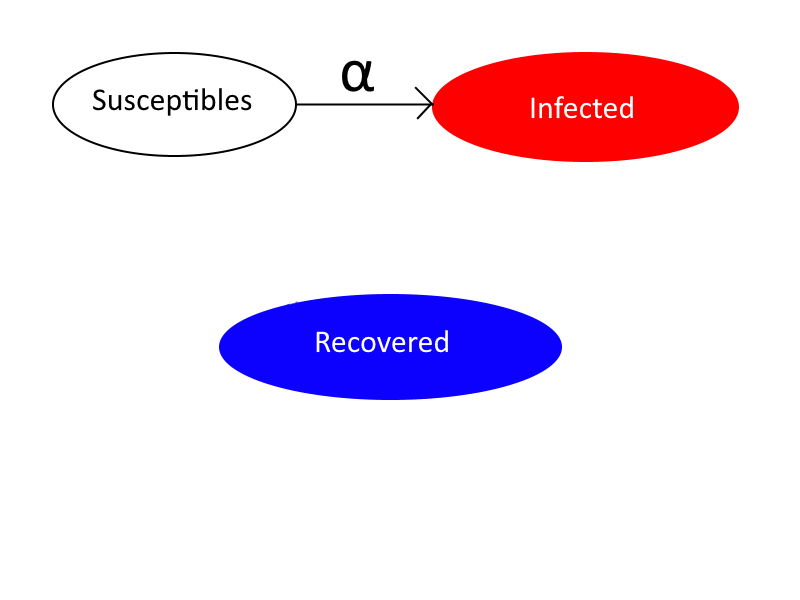
\includegraphics[width=\columnwidth]{MySIR}
		\label{fig:MySIR}
	\end{figure}

	Ces états, susceptibles, infectés, et retirés, représentent respectivement la population saine, la population malade et contagieuse, et la population vaccinée. $\alpha$ représente la probabilité qu'un individu sain se fasse infecté.
	Ce modèle seul ne permet pas de simuler de manière satisfaisante et représentative l'évolution dans une population, nous l'avons donc adapté dans un modèle spatial décrit en \ref{sec:modele_spatial}


	\subsection{Modèle spatial}
	\label{sec:modele_spatial}
	Ce modèle se base sur la représentation d'une population de 2500 individus sur un plan en 2 dimensions. Chaque individu est représenté par un point sur une matrice carrée de 50 points de côtés, ne peut être dans un état à la fois, et est voisin de 8 autres individus. Un individu ne peut infecter que quelqu'un dont il est voisin. Un malade contagieux ne pourra donc pas infecter plus de 8 individus ($R_0 \leq 8$)
	D'abord tous les individus commencent susceptibles, puis, avant le début de l'infection, une proportion fixée de la population est vacciné, puis, une personne susceptible au hasard est sélectionnée pour être l'infecté de départ (Le programme Python avec interface graphique que nous avons écrit permet de faire varier ces paramètres)
	\subsubsection{La vaccination}
	Un taux fixé de la population est vacciné avant l'apparition d'un patient zéro. Une vaccination ne peut s'effectuer que sur un individu susceptible et ce vaccin est efficace à 100\%. Cependant, il existe bon nombre de modèles prenant en compte les différentes mécanismes qui peuvent empêcher un vaccin de fonctionner \cite{Crowcroft_Klein_2018}. Cette efficacité à 100\% n'est bien sûr pas une représentation de la réalité, mais une simplification du phénomène complexe qu'est la vaccination
	\subsubsection{L'infection de départ}
	Parmi les personnes saines dans la population, nous sélectionnons une personne au hasard pour démarrer l'épidémie. Cette personne infectée sera immédiatement contagieuse et chaque personne infectée dans le futur sera aussi immédiatement contagieuse. Dans la réalité, il existe une période d'incubation ainsi qu'une période de transmission (qui peuvent ou pas se chevaucher) mais nous avons choisi d'ignorer ces phénomènes afin de simplifier le modèle.
	\subsubsection{La guérison}
	Un individu ne guéri pas. En effet cet article se concentre sur l'infection des individus dans une population vaccinée, il n'est donc pas pertinant de tenir compte de la guérison des individus, nous voulons juste connaitre l'amplitude de l'épidémie en nombre d'infectés
	\subsubsection{La propagation}
	Pour chaque voisin susceptible de chaque individu infecté, nous l'infectons avec une probabilité de $\alpha$. Dans le cadre de ce projet, nous avons choisi un $\alpha$ de $1$ car nous voulions voir l'évolution d'une maladie très infectieuse, évoluant donc rapidement avec le temps. Choisir une valeur de $\alpha < 1$ ne serait pas utile dans cette étude étant donné qu'il n'y a que une transition dans le modèle, diminuer le taux de transition revient donc simplement à ralentir la simulation.
	\subsubsection{Probabilité de propagation et isolement}
	Au vu de la construction de notre modèle spatiale, il existe des cas particuliers empêchant totalement la propagation de la maladie, par exemple si un individu est entouré de 8 individus vacciné.
	La probabilité qu'un individu ai k voisins vaccinés est représentée par la figure \ref{fig:probNeighbour}
	Cette probabilité est calculée en utilisant une binomiale. En effet, la probabilité d'avoir k voisins vacciné lorsque la probabilité d'être vacciné est de p, est égale au fait de réussir k événement ``recevoir un vaccin'' en n (nombre de voisins) tentatives avec une probabilité de p de réussite de l'événement. Nous avons donc l'équation \ref{eqn:binomial}
	\begin{equation}
		\label{eqn:binomial}
		\begin{aligned}
			P(X = k) = B(n;p) = {n \choose k}\times p^k \times (1-p)^{n-k} = \\ \frac{n!}{k!(n-k)!}\times p^k \times (1-p)^{n-k}
		\end{aligned}
	\end{equation}
	où X est la variable aléatoire ``Nombre de voisins vaccinés'', k le nombre de voisins vaccinés (entre 1 et 8), p la probabilité pour un individu d'être vacciné, et n le nombre de voisins, 8 dans notre simulation. En calculant cette valeur pour tous les pourcentages de vaccination et pour tous les nombres de voisins vaccinés de 1 à 8, nous obtenons ce graphe

	\begin{figure}[!hbt]
		\caption{Probabilité d'avoir x voisins vaccinés en fonction du pourcentage de vaccinés}
		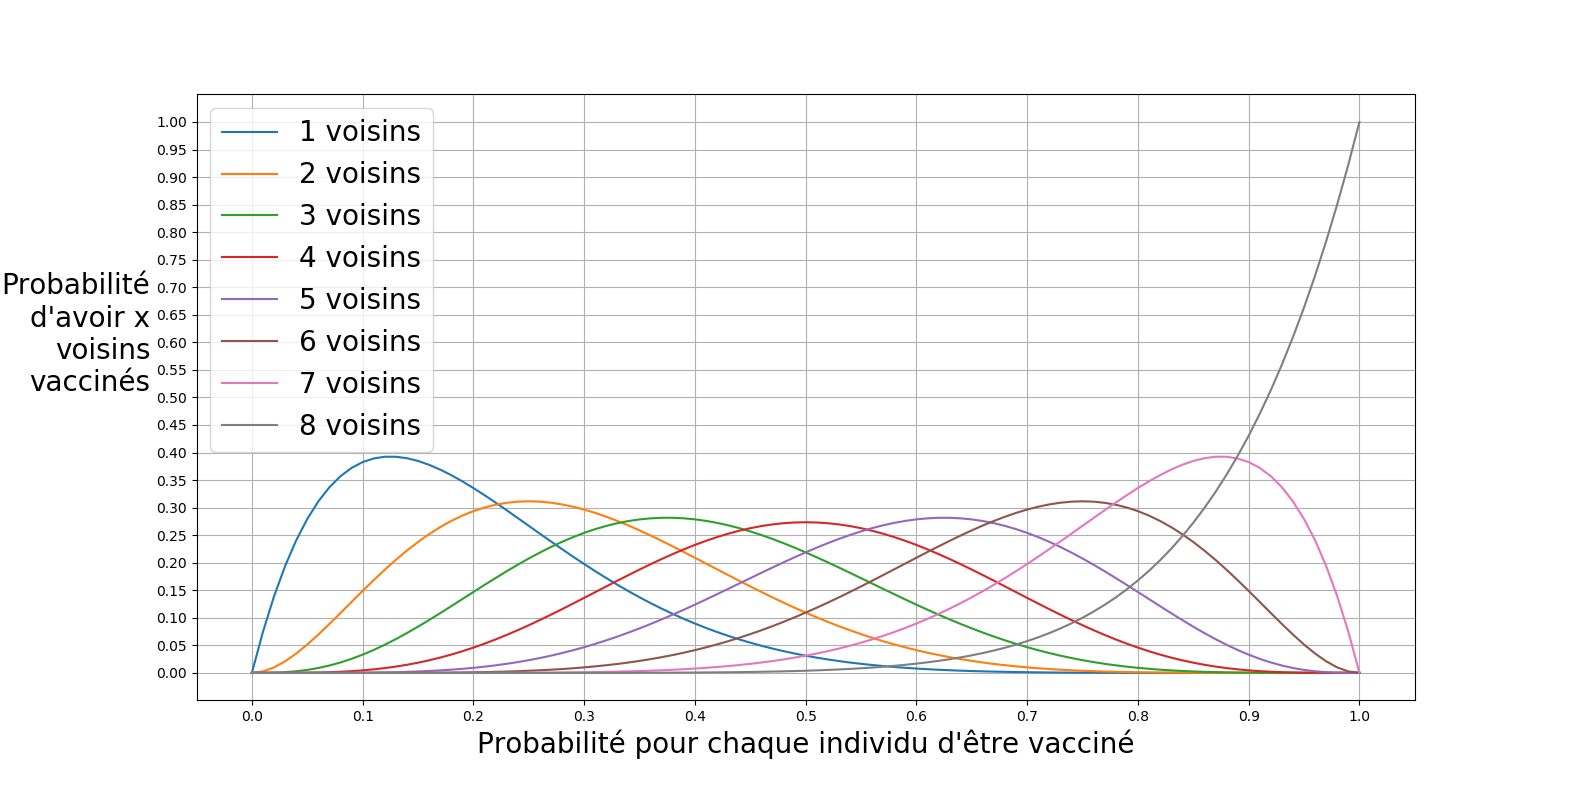
\includegraphics[width=\columnwidth]{probNeighbour}
		\label{fig:probNeighbour}
	\end{figure}

	Nous voyons donc que lorsque la population est vaccinée à 90\%, il y a déjà plus de 40\% des individus qui sont totalement isolés de la maladie. Il s'agit donc de 40\% d'individus qui n'attraperont jamais la maladie ce qui réduit automatiquement le taux de personnes infecté à la fin de l'épidémie. Cette immunité par isolement n'apporte malheureusement que trop peu de protection que pour être considéré comme un moyen efficace de protéger la population. Cette immunité part du principe que la vaccination agisse comme une sorte de barrière \cite{vaccine_as_barrier}

	\subsubsection{Seuil d'Immunité Grégaire (HIT)}
	Ce seuil d'immunité est dépend de $R_0$, le nombre d'individus qu'un malade infecte en moyenne. Si ce nombre est inférieur à 1, alors la maladie finira par s'éteindre, si il est supérieur à 1, la maladie infectera tout le monde si rien n'est fait pour l'arrêter.
	Le taux de reproduction effectif, noté $R_t = R_0 \times (1-P)$ quant à lui est une mesure du nombre d'individu qu'un malade infecte au temps t, c'est-à-dire en tenant compte des ``barrières''(vaccins, quarantaine, etc...), mais aussi de la mortalité et de la contagion de la maladie. $P$ est la proportion d'individus vaccinés. Le taux de reproduction effectif $R_t$ sera inférieur à 1 pour autant que la valeur de P soit supérieure à $1-1/R_0$ \cite{herd_guide}. Un individu malade contaminera alors en moyenne moins d'une personne ce qui finira par faire tomber le nombre de malades à 0 pour peu que les malades guérissent ou meurt. Il faut donc vacciner une proportion de la population égale à $1-\frac{1}{R_0}$ pour qu'un malade ne puisse plus infecter, en moyenne, qu'une personne dans son entourage.\\
	Dans le cadre de notre modèle, ce taux est donc de $0.875$. Ce qui signifie que, en moyenne, dans une population infinie, si chaque individu est vacciné avec une probabilité de 0.875, la maladie se transmettrait un individu à la fois et ne s'arrêterait que lorsque toute la population aura été touchée. A $0.875+\epsilon$ de la population vaccinée, la maladie se hurterait à un moment sur une personne qui n'a aucun voisin susceptible et s'arrêtera donc là. Plus $\epsilon$ est grand, plus ce moment arrivera vite après l'infection du patient zéro



% Main Part
\section{Résultats}
	Nous obtenons ainsi une courbe en S liant le taux de vaccination, sur l'axe des abscisses, au taux de protection des individus non-vaccinés, sur l'axe des ordonées sur la figure \ref{fig:results}.
	\begin{figure}[!hbt]
	\caption{Efficacité de la couverture vaccinale sur les individus non vaccinés}
		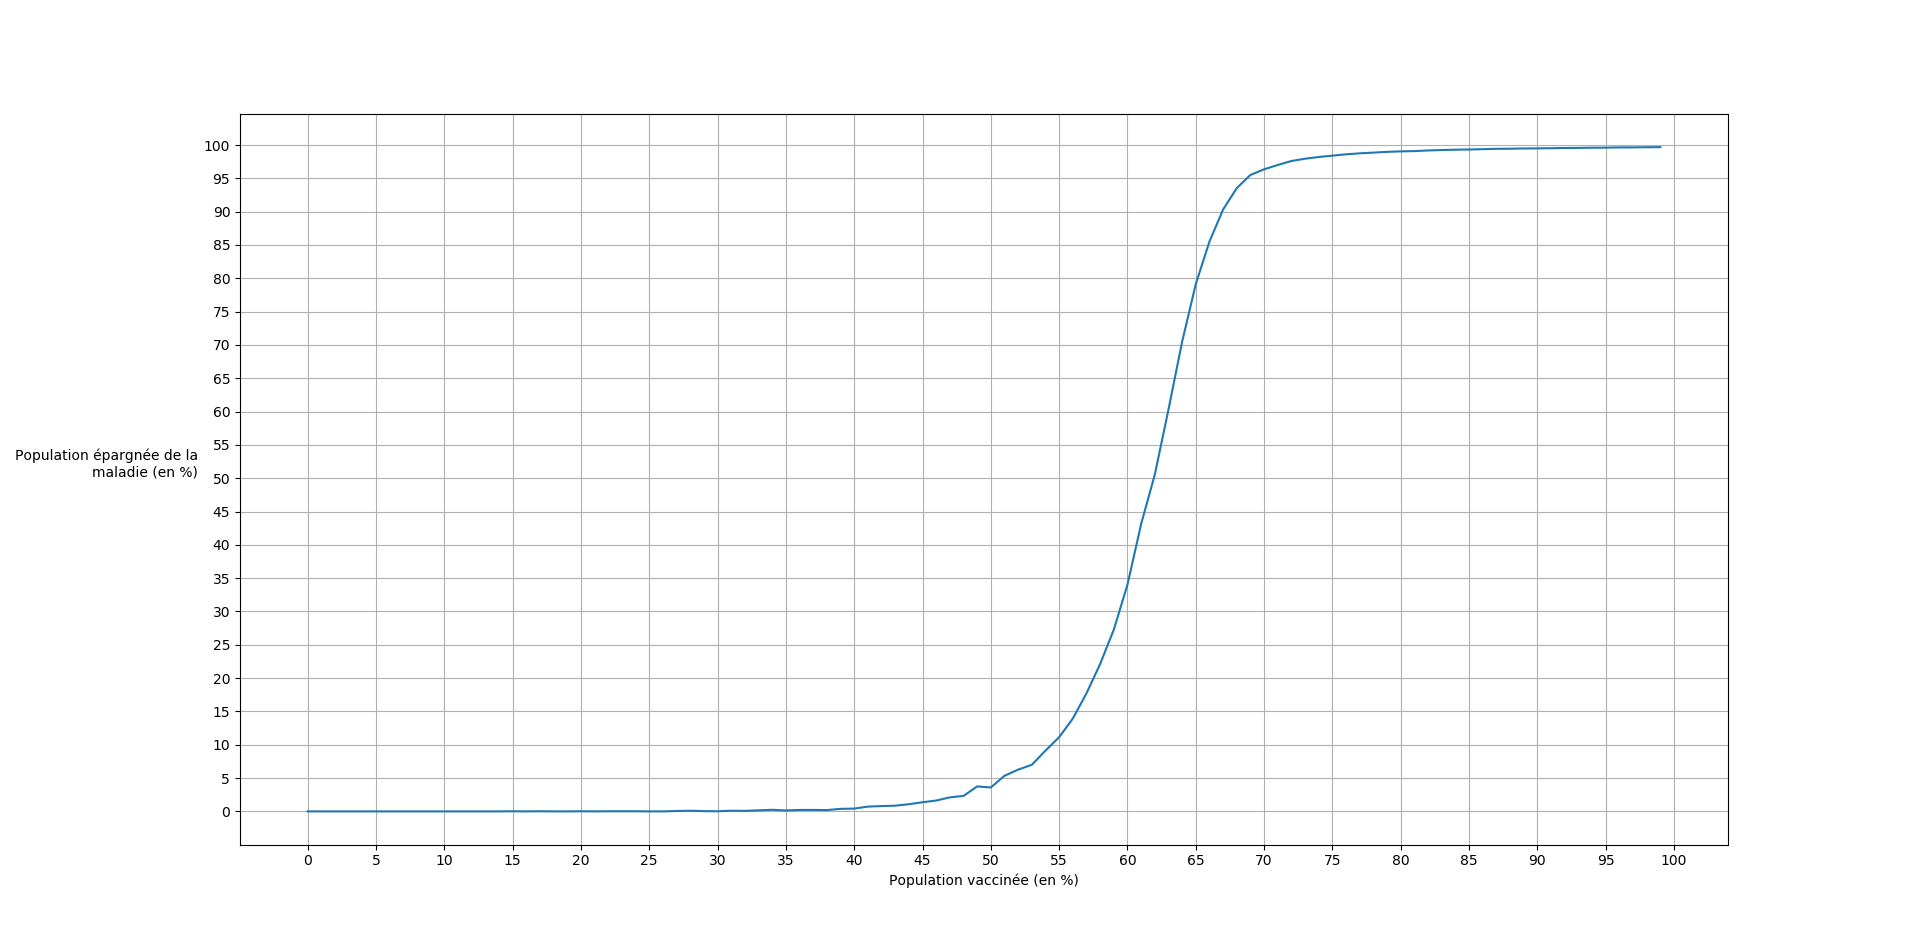
\includegraphics[width=\columnwidth]{Results}
		\label{fig:results}
	\end{figure}
 On remarque que vacciner une population à seulement environ 40\% est inefficace pour empêcher une maladie de se répandre. Par contre, entre 40 et 75\%, chaque personne vacciné compte au vu de la croissance ultra-rapide de la courbe entre ces deux valeurs. Enfin on peut aussi remarquer qu'à 85\%, presque toute la population est protégée, du moins dans le cadre de cette simulation. \\
	En effet, cette simulation étant basée sur un modèle SIR assez simple, elle ne tient pas en compte de tout un tas de cas de transmissions dans la réalité comme par exemple les déplacements d'individus dans la population, les transmissions indirectes par l'environnement, ...
	Par contre, la simulation ne tient pas non plus compte des actions qui entravent la transmission comme la mise en quarantaine, les gestes barrières, ...
	Ces actions ont tendance à diminuer ou augmenter la valeur de $R_t$ qui modifie donc la courbe d'efficacité vaccinale sur la figure \ref{fig:results}. Un modèle avec beaucoup plus de cas de transmission sera forcément plus pessimiste qu'un modèle prenant en compte une population faisant de son mieux pour arrêter l'épidémie. Augmenter le réalisme des modèle, et donc réduire la marge d'erreur des résultats, demande une puissance de calcul supplémentaire dont on ne pouvait pas se permettre pour générer dans les temps assez de résultats pour tracer la figure \ref{fig:results}



\section{Conclusion}
Cette simulation reste assez loin de la réalité du fait qu'elle ai si peu d'états et de transmissions et qu'elle ignore beaucoup de phénomène modélisables (efficacité du vaccin, période d'incubations et transmissions, mouvement des foules etc). Cependant il était quand même très intéressant de construire ce programme afin de voir émerger une telle complexité de l'immunité des individus non vaccinés avec des règles de transmissions assez simple.\\
Nous allons donc voir ici comment nous aurions pu implémenter des modifications afin de rendre notre modèle plus réaliste
\subsection{Efficacité du vaccin}
En injectant le contenu d'une seringue à quelqu'un, nous ne pouvons pas être sûr que cette personne soit protégée à 100\% du microbe. Nous pourrions donc crée un état vacciné avec une transition de susceptible vers vacciné et de vacciné vers infecté et vers guéri. Un individu vacciné serait alors toujours susceptible selon un paramètre d'efficacité du vaccin mais pourrait aussi être considéré guéri selon le même paramètre (probabilité complémentaire).
\subsection{Période d'incubation et de transmission}
Un individu infecté n'est pas immédiatement contagieux dans un grand nombre de cas. On pourrait donc changer notre modèle SIR en modèle SEIR en rajoutant l'était Exposé (à la maladie). Un individu susceptible ne pourrait alors plus être infecté mais serait d'abord exposé un certain temps avant d'être infecté et contagieux. L'ajout de ce nouvel état à notre simulation telle quelle ne ferait que ralentir l'épidémie du fait qu'un individu précédemment susceptible mettrait plusieurs unités de temps avant de transmettre la maladie contre 1 seule dans notre programme.
\subsection{Quarantaine}
Pendant les périodes d'épidémie, il peut être intéressant d'utiliser la quarantaine comme \textit{moyen de vaccination}. En effet être en quarantaine à le même effet qu'être vacciné, du point de vue de notre modèle. Un individu en quarantaine c'est un individu qui ne peut ni transmettre, ni être infecté.
Nous pourrions rajouter à notre modèle un état de quarantaine ainsi qu'une transition entre infecté et quarantaine. Un individu infecté possède une certaine probabilité d'être mis en quarantaine, un état duquel il ne peut plus infecter d'individus. La transition vers quarantaine pourrait aussi se faire depuis les individus susceptibles ou exposés qui se mettraient d'eux-même en quarantaine pour se protéger soi et pour protéger la population.

% Cette section contient un rappel des contributions / de résultats importants de votre article et éventuellement une indication sur les perspectives de recherche future dans le même domaine.


\bibliographystyle{unsrt}
\bibliography{bibliography}

\newpage

% Your document ends here!
\end{document}
